\section{second closed-loop simulation}

\subsection{Simulink diagram}
	\begin{figure}[H]
		\centering
		\begin{subfigure}[b]{0.7\textwidth}
			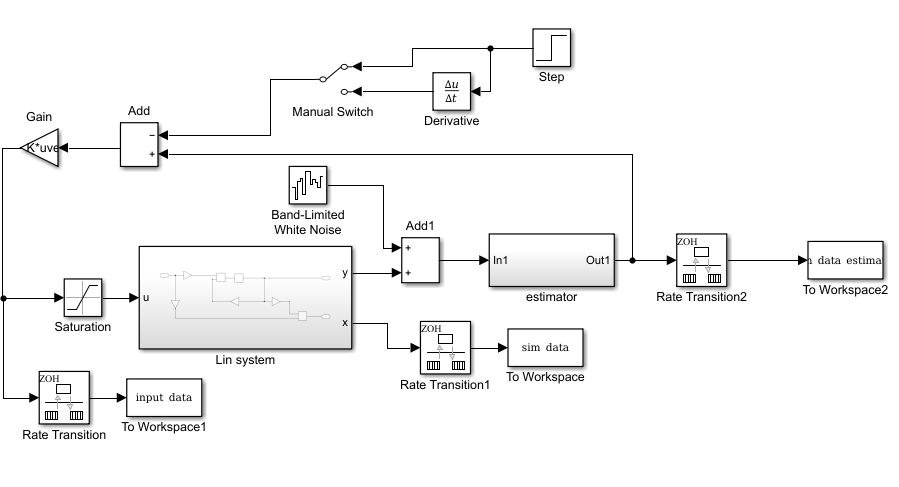
\includegraphics[width=\textwidth]{./part3_LQR2/not_generated/simulink_main.png}
			\caption{main diagram simulink}
		\end{subfigure}
		\begin{subfigure}[b]{0.45\textwidth}
			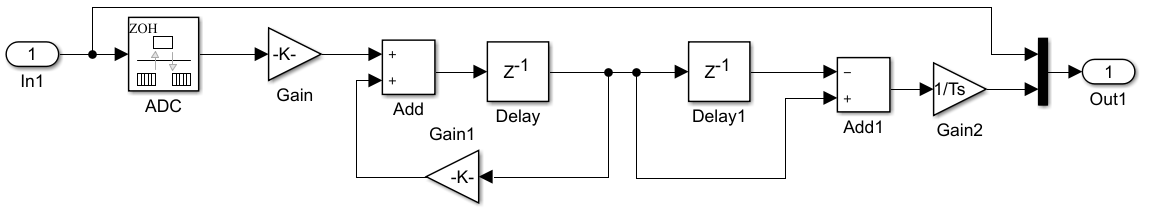
\includegraphics[width=\textwidth]{./part3_LQR2/not_generated/simulink_estimator.png}
			\caption{estimator}
		\end{subfigure}
		\begin{subfigure}[b]{0.45\textwidth}
			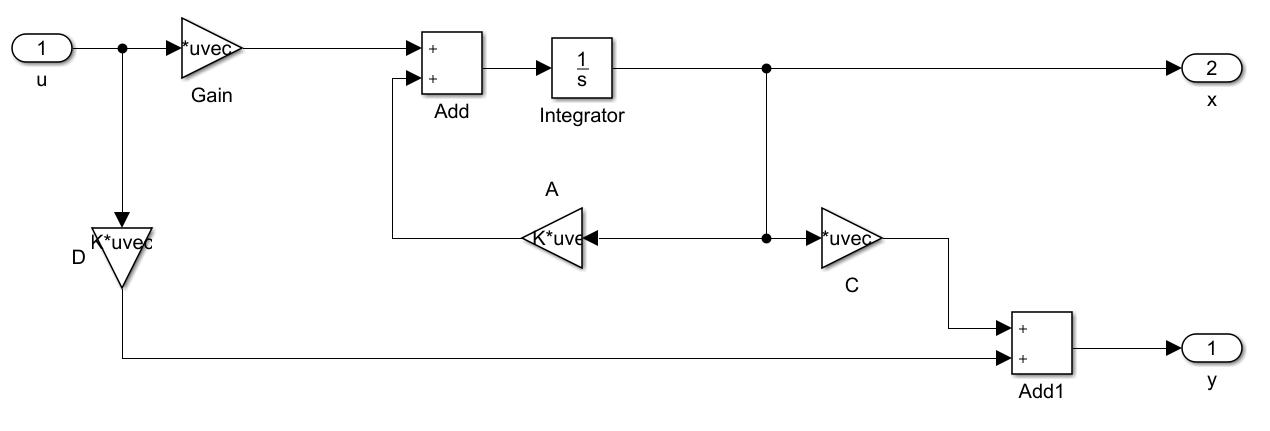
\includegraphics[width=\textwidth]{./part3_LQR2/not_generated/simulink_lin_sys.png}
			\caption{linear system}
		\end{subfigure}
		\caption{simulink diagrams}
	\end{figure}
\subsection{simulation with noise}
	\begin{figure}[H]
		\centering
		\begin{subfigure}[b]{0.45\textwidth}
			\includegraphics[width=\textwidth]{./part3_LQR2/normal_parameters_estimated_states.png}
			\caption{estimated states}
		\end{subfigure}
		\begin{subfigure}[b]{0.45\textwidth}
			\includegraphics[width=\textwidth]{./part3_LQR2/normal_parameters_states.png}
			\caption{real states}
		\end{subfigure}
		\begin{subfigure}[b]{0.45\textwidth}
			\includegraphics[width=\textwidth]{./part3_LQR2/normal_parameters_input.png}
			\caption{input to motor}
		\end{subfigure}
		\caption{simulation results with a noise with power=$10^{-8}$}
	\end{figure}
\subsection{simulation with noise from experiments}
	\begin{figure}[H]
		\centering
		\begin{subfigure}[b]{0.45\textwidth}
			\includegraphics[width=\textwidth]{./part3_LQR2/noise_experiments_estimated_states.png}
			\caption{estimated states}
		\end{subfigure}
		\begin{subfigure}[b]{0.45\textwidth}
			\includegraphics[width=\textwidth]{./part3_LQR2/noise_experiments_states.png}
			\caption{real states}
		\end{subfigure}
		\begin{subfigure}[b]{0.45\textwidth}
			\includegraphics[width=\textwidth]{./part3_LQR2/noise_experiments_input.png}
			\caption{input to motor}
		\end{subfigure}
		\caption{simulation results with noise derived from experiments}
	\end{figure}
\subsection{determining the cutt-off frequency}
\subsection{investigating the role of the cut-off frequency}